\documentclass{article} % For LaTeX2e
\usepackage{iclr2026,times}

% Optional math commands from https://github.com/goodfeli/dlbook_notation.
%%%%% NEW MATH DEFINITIONS %%%%%

\usepackage{amsmath,amsfonts,bm}

% Mark sections of captions for referring to divisions of figures
\newcommand{\figleft}{{\em (Left)}}
\newcommand{\figcenter}{{\em (Center)}}
\newcommand{\figright}{{\em (Right)}}
\newcommand{\figtop}{{\em (Top)}}
\newcommand{\figbottom}{{\em (Bottom)}}
\newcommand{\captiona}{{\em (a)}}
\newcommand{\captionb}{{\em (b)}}
\newcommand{\captionc}{{\em (c)}}
\newcommand{\captiond}{{\em (d)}}

% Highlight a newly defined term
\newcommand{\newterm}[1]{{\bf #1}}


% Figure reference, lower-case.
\def\figref#1{figure~\ref{#1}}
% Figure reference, capital. For start of sentence
\def\Figref#1{Figure~\ref{#1}}
\def\twofigref#1#2{figures \ref{#1} and \ref{#2}}
\def\quadfigref#1#2#3#4{figures \ref{#1}, \ref{#2}, \ref{#3} and \ref{#4}}
% Section reference, lower-case.
\def\secref#1{section~\ref{#1}}
% Section reference, capital.
\def\Secref#1{Section~\ref{#1}}
% Reference to two sections.
\def\twosecrefs#1#2{sections \ref{#1} and \ref{#2}}
% Reference to three sections.
\def\secrefs#1#2#3{sections \ref{#1}, \ref{#2} and \ref{#3}}
% Reference to an equation, lower-case.
\def\eqref#1{equation~\ref{#1}}
% Reference to an equation, upper case
\def\Eqref#1{Equation~\ref{#1}}
% A raw reference to an equation---avoid using if possible
\def\plaineqref#1{\ref{#1}}
% Reference to a chapter, lower-case.
\def\chapref#1{chapter~\ref{#1}}
% Reference to an equation, upper case.
\def\Chapref#1{Chapter~\ref{#1}}
% Reference to a range of chapters
\def\rangechapref#1#2{chapters\ref{#1}--\ref{#2}}
% Reference to an algorithm, lower-case.
\def\algref#1{algorithm~\ref{#1}}
% Reference to an algorithm, upper case.
\def\Algref#1{Algorithm~\ref{#1}}
\def\twoalgref#1#2{algorithms \ref{#1} and \ref{#2}}
\def\Twoalgref#1#2{Algorithms \ref{#1} and \ref{#2}}
% Reference to a part, lower case
\def\partref#1{part~\ref{#1}}
% Reference to a part, upper case
\def\Partref#1{Part~\ref{#1}}
\def\twopartref#1#2{parts \ref{#1} and \ref{#2}}

\def\ceil#1{\lceil #1 \rceil}
\def\floor#1{\lfloor #1 \rfloor}
\def\1{\bm{1}}
\newcommand{\train}{\mathcal{D}}
\newcommand{\valid}{\mathcal{D_{\mathrm{valid}}}}
\newcommand{\test}{\mathcal{D_{\mathrm{test}}}}

\def\eps{{\epsilon}}


% Random variables
\def\reta{{\textnormal{$\eta$}}}
\def\ra{{\textnormal{a}}}
\def\rb{{\textnormal{b}}}
\def\rc{{\textnormal{c}}}
\def\rd{{\textnormal{d}}}
\def\re{{\textnormal{e}}}
\def\rf{{\textnormal{f}}}
\def\rg{{\textnormal{g}}}
\def\rh{{\textnormal{h}}}
\def\ri{{\textnormal{i}}}
\def\rj{{\textnormal{j}}}
\def\rk{{\textnormal{k}}}
\def\rl{{\textnormal{l}}}
% rm is already a command, just don't name any random variables m
\def\rn{{\textnormal{n}}}
\def\ro{{\textnormal{o}}}
\def\rp{{\textnormal{p}}}
\def\rq{{\textnormal{q}}}
\def\rr{{\textnormal{r}}}
\def\rs{{\textnormal{s}}}
\def\rt{{\textnormal{t}}}
\def\ru{{\textnormal{u}}}
\def\rv{{\textnormal{v}}}
\def\rw{{\textnormal{w}}}
\def\rx{{\textnormal{x}}}
\def\ry{{\textnormal{y}}}
\def\rz{{\textnormal{z}}}

% Random vectors
\def\rvepsilon{{\mathbf{\epsilon}}}
\def\rvtheta{{\mathbf{\theta}}}
\def\rva{{\mathbf{a}}}
\def\rvb{{\mathbf{b}}}
\def\rvc{{\mathbf{c}}}
\def\rvd{{\mathbf{d}}}
\def\rve{{\mathbf{e}}}
\def\rvf{{\mathbf{f}}}
\def\rvg{{\mathbf{g}}}
\def\rvh{{\mathbf{h}}}
\def\rvu{{\mathbf{i}}}
\def\rvj{{\mathbf{j}}}
\def\rvk{{\mathbf{k}}}
\def\rvl{{\mathbf{l}}}
\def\rvm{{\mathbf{m}}}
\def\rvn{{\mathbf{n}}}
\def\rvo{{\mathbf{o}}}
\def\rvp{{\mathbf{p}}}
\def\rvq{{\mathbf{q}}}
\def\rvr{{\mathbf{r}}}
\def\rvs{{\mathbf{s}}}
\def\rvt{{\mathbf{t}}}
\def\rvu{{\mathbf{u}}}
\def\rvv{{\mathbf{v}}}
\def\rvw{{\mathbf{w}}}
\def\rvx{{\mathbf{x}}}
\def\rvy{{\mathbf{y}}}
\def\rvz{{\mathbf{z}}}

% Elements of random vectors
\def\erva{{\textnormal{a}}}
\def\ervb{{\textnormal{b}}}
\def\ervc{{\textnormal{c}}}
\def\ervd{{\textnormal{d}}}
\def\erve{{\textnormal{e}}}
\def\ervf{{\textnormal{f}}}
\def\ervg{{\textnormal{g}}}
\def\ervh{{\textnormal{h}}}
\def\ervi{{\textnormal{i}}}
\def\ervj{{\textnormal{j}}}
\def\ervk{{\textnormal{k}}}
\def\ervl{{\textnormal{l}}}
\def\ervm{{\textnormal{m}}}
\def\ervn{{\textnormal{n}}}
\def\ervo{{\textnormal{o}}}
\def\ervp{{\textnormal{p}}}
\def\ervq{{\textnormal{q}}}
\def\ervr{{\textnormal{r}}}
\def\ervs{{\textnormal{s}}}
\def\ervt{{\textnormal{t}}}
\def\ervu{{\textnormal{u}}}
\def\ervv{{\textnormal{v}}}
\def\ervw{{\textnormal{w}}}
\def\ervx{{\textnormal{x}}}
\def\ervy{{\textnormal{y}}}
\def\ervz{{\textnormal{z}}}

% Random matrices
\def\rmA{{\mathbf{A}}}
\def\rmB{{\mathbf{B}}}
\def\rmC{{\mathbf{C}}}
\def\rmD{{\mathbf{D}}}
\def\rmE{{\mathbf{E}}}
\def\rmF{{\mathbf{F}}}
\def\rmG{{\mathbf{G}}}
\def\rmH{{\mathbf{H}}}
\def\rmI{{\mathbf{I}}}
\def\rmJ{{\mathbf{J}}}
\def\rmK{{\mathbf{K}}}
\def\rmL{{\mathbf{L}}}
\def\rmM{{\mathbf{M}}}
\def\rmN{{\mathbf{N}}}
\def\rmO{{\mathbf{O}}}
\def\rmP{{\mathbf{P}}}
\def\rmQ{{\mathbf{Q}}}
\def\rmR{{\mathbf{R}}}
\def\rmS{{\mathbf{S}}}
\def\rmT{{\mathbf{T}}}
\def\rmU{{\mathbf{U}}}
\def\rmV{{\mathbf{V}}}
\def\rmW{{\mathbf{W}}}
\def\rmX{{\mathbf{X}}}
\def\rmY{{\mathbf{Y}}}
\def\rmZ{{\mathbf{Z}}}

% Elements of random matrices
\def\ermA{{\textnormal{A}}}
\def\ermB{{\textnormal{B}}}
\def\ermC{{\textnormal{C}}}
\def\ermD{{\textnormal{D}}}
\def\ermE{{\textnormal{E}}}
\def\ermF{{\textnormal{F}}}
\def\ermG{{\textnormal{G}}}
\def\ermH{{\textnormal{H}}}
\def\ermI{{\textnormal{I}}}
\def\ermJ{{\textnormal{J}}}
\def\ermK{{\textnormal{K}}}
\def\ermL{{\textnormal{L}}}
\def\ermM{{\textnormal{M}}}
\def\ermN{{\textnormal{N}}}
\def\ermO{{\textnormal{O}}}
\def\ermP{{\textnormal{P}}}
\def\ermQ{{\textnormal{Q}}}
\def\ermR{{\textnormal{R}}}
\def\ermS{{\textnormal{S}}}
\def\ermT{{\textnormal{T}}}
\def\ermU{{\textnormal{U}}}
\def\ermV{{\textnormal{V}}}
\def\ermW{{\textnormal{W}}}
\def\ermX{{\textnormal{X}}}
\def\ermY{{\textnormal{Y}}}
\def\ermZ{{\textnormal{Z}}}

% Vectors
\def\vzero{{\bm{0}}}
\def\vone{{\bm{1}}}
\def\vmu{{\bm{\mu}}}
\def\vtheta{{\bm{\theta}}}
\def\va{{\bm{a}}}
\def\vb{{\bm{b}}}
\def\vc{{\bm{c}}}
\def\vd{{\bm{d}}}
\def\ve{{\bm{e}}}
\def\vf{{\bm{f}}}
\def\vg{{\bm{g}}}
\def\vh{{\bm{h}}}
\def\vi{{\bm{i}}}
\def\vj{{\bm{j}}}
\def\vk{{\bm{k}}}
\def\vl{{\bm{l}}}
\def\vm{{\bm{m}}}
\def\vn{{\bm{n}}}
\def\vo{{\bm{o}}}
\def\vp{{\bm{p}}}
\def\vq{{\bm{q}}}
\def\vr{{\bm{r}}}
\def\vs{{\bm{s}}}
\def\vt{{\bm{t}}}
\def\vu{{\bm{u}}}
\def\vv{{\bm{v}}}
\def\vw{{\bm{w}}}
\def\vx{{\bm{x}}}
\def\vy{{\bm{y}}}
\def\vz{{\bm{z}}}

% Elements of vectors
\def\evalpha{{\alpha}}
\def\evbeta{{\beta}}
\def\evepsilon{{\epsilon}}
\def\evlambda{{\lambda}}
\def\evomega{{\omega}}
\def\evmu{{\mu}}
\def\evpsi{{\psi}}
\def\evsigma{{\sigma}}
\def\evtheta{{\theta}}
\def\eva{{a}}
\def\evb{{b}}
\def\evc{{c}}
\def\evd{{d}}
\def\eve{{e}}
\def\evf{{f}}
\def\evg{{g}}
\def\evh{{h}}
\def\evi{{i}}
\def\evj{{j}}
\def\evk{{k}}
\def\evl{{l}}
\def\evm{{m}}
\def\evn{{n}}
\def\evo{{o}}
\def\evp{{p}}
\def\evq{{q}}
\def\evr{{r}}
\def\evs{{s}}
\def\evt{{t}}
\def\evu{{u}}
\def\evv{{v}}
\def\evw{{w}}
\def\evx{{x}}
\def\evy{{y}}
\def\evz{{z}}

% Matrix
\def\mA{{\bm{A}}}
\def\mB{{\bm{B}}}
\def\mC{{\bm{C}}}
\def\mD{{\bm{D}}}
\def\mE{{\bm{E}}}
\def\mF{{\bm{F}}}
\def\mG{{\bm{G}}}
\def\mH{{\bm{H}}}
\def\mI{{\bm{I}}}
\def\mJ{{\bm{J}}}
\def\mK{{\bm{K}}}
\def\mL{{\bm{L}}}
\def\mM{{\bm{M}}}
\def\mN{{\bm{N}}}
\def\mO{{\bm{O}}}
\def\mP{{\bm{P}}}
\def\mQ{{\bm{Q}}}
\def\mR{{\bm{R}}}
\def\mS{{\bm{S}}}
\def\mT{{\bm{T}}}
\def\mU{{\bm{U}}}
\def\mV{{\bm{V}}}
\def\mW{{\bm{W}}}
\def\mX{{\bm{X}}}
\def\mY{{\bm{Y}}}
\def\mZ{{\bm{Z}}}
\def\mBeta{{\bm{\beta}}}
\def\mPhi{{\bm{\Phi}}}
\def\mLambda{{\bm{\Lambda}}}
\def\mSigma{{\bm{\Sigma}}}

% Tensor
\DeclareMathAlphabet{\mathsfit}{\encodingdefault}{\sfdefault}{m}{sl}
\SetMathAlphabet{\mathsfit}{bold}{\encodingdefault}{\sfdefault}{bx}{n}
\newcommand{\tens}[1]{\bm{\mathsfit{#1}}}
\def\tA{{\tens{A}}}
\def\tB{{\tens{B}}}
\def\tC{{\tens{C}}}
\def\tD{{\tens{D}}}
\def\tE{{\tens{E}}}
\def\tF{{\tens{F}}}
\def\tG{{\tens{G}}}
\def\tH{{\tens{H}}}
\def\tI{{\tens{I}}}
\def\tJ{{\tens{J}}}
\def\tK{{\tens{K}}}
\def\tL{{\tens{L}}}
\def\tM{{\tens{M}}}
\def\tN{{\tens{N}}}
\def\tO{{\tens{O}}}
\def\tP{{\tens{P}}}
\def\tQ{{\tens{Q}}}
\def\tR{{\tens{R}}}
\def\tS{{\tens{S}}}
\def\tT{{\tens{T}}}
\def\tU{{\tens{U}}}
\def\tV{{\tens{V}}}
\def\tW{{\tens{W}}}
\def\tX{{\tens{X}}}
\def\tY{{\tens{Y}}}
\def\tZ{{\tens{Z}}}


% Graph
\def\gA{{\mathcal{A}}}
\def\gB{{\mathcal{B}}}
\def\gC{{\mathcal{C}}}
\def\gD{{\mathcal{D}}}
\def\gE{{\mathcal{E}}}
\def\gF{{\mathcal{F}}}
\def\gG{{\mathcal{G}}}
\def\gH{{\mathcal{H}}}
\def\gI{{\mathcal{I}}}
\def\gJ{{\mathcal{J}}}
\def\gK{{\mathcal{K}}}
\def\gL{{\mathcal{L}}}
\def\gM{{\mathcal{M}}}
\def\gN{{\mathcal{N}}}
\def\gO{{\mathcal{O}}}
\def\gP{{\mathcal{P}}}
\def\gQ{{\mathcal{Q}}}
\def\gR{{\mathcal{R}}}
\def\gS{{\mathcal{S}}}
\def\gT{{\mathcal{T}}}
\def\gU{{\mathcal{U}}}
\def\gV{{\mathcal{V}}}
\def\gW{{\mathcal{W}}}
\def\gX{{\mathcal{X}}}
\def\gY{{\mathcal{Y}}}
\def\gZ{{\mathcal{Z}}}

% Sets
\def\sA{{\mathbb{A}}}
\def\sB{{\mathbb{B}}}
\def\sC{{\mathbb{C}}}
\def\sD{{\mathbb{D}}}
% Don't use a set called E, because this would be the same as our symbol
% for expectation.
\def\sF{{\mathbb{F}}}
\def\sG{{\mathbb{G}}}
\def\sH{{\mathbb{H}}}
\def\sI{{\mathbb{I}}}
\def\sJ{{\mathbb{J}}}
\def\sK{{\mathbb{K}}}
\def\sL{{\mathbb{L}}}
\def\sM{{\mathbb{M}}}
\def\sN{{\mathbb{N}}}
\def\sO{{\mathbb{O}}}
\def\sP{{\mathbb{P}}}
\def\sQ{{\mathbb{Q}}}
\def\sR{{\mathbb{R}}}
\def\sS{{\mathbb{S}}}
\def\sT{{\mathbb{T}}}
\def\sU{{\mathbb{U}}}
\def\sV{{\mathbb{V}}}
\def\sW{{\mathbb{W}}}
\def\sX{{\mathbb{X}}}
\def\sY{{\mathbb{Y}}}
\def\sZ{{\mathbb{Z}}}

% Entries of a matrix
\def\emLambda{{\Lambda}}
\def\emA{{A}}
\def\emB{{B}}
\def\emC{{C}}
\def\emD{{D}}
\def\emE{{E}}
\def\emF{{F}}
\def\emG{{G}}
\def\emH{{H}}
\def\emI{{I}}
\def\emJ{{J}}
\def\emK{{K}}
\def\emL{{L}}
\def\emM{{M}}
\def\emN{{N}}
\def\emO{{O}}
\def\emP{{P}}
\def\emQ{{Q}}
\def\emR{{R}}
\def\emS{{S}}
\def\emT{{T}}
\def\emU{{U}}
\def\emV{{V}}
\def\emW{{W}}
\def\emX{{X}}
\def\emY{{Y}}
\def\emZ{{Z}}
\def\emSigma{{\Sigma}}

% entries of a tensor
% Same font as tensor, without \bm wrapper
\newcommand{\etens}[1]{\mathsfit{#1}}
\def\etLambda{{\etens{\Lambda}}}
\def\etA{{\etens{A}}}
\def\etB{{\etens{B}}}
\def\etC{{\etens{C}}}
\def\etD{{\etens{D}}}
\def\etE{{\etens{E}}}
\def\etF{{\etens{F}}}
\def\etG{{\etens{G}}}
\def\etH{{\etens{H}}}
\def\etI{{\etens{I}}}
\def\etJ{{\etens{J}}}
\def\etK{{\etens{K}}}
\def\etL{{\etens{L}}}
\def\etM{{\etens{M}}}
\def\etN{{\etens{N}}}
\def\etO{{\etens{O}}}
\def\etP{{\etens{P}}}
\def\etQ{{\etens{Q}}}
\def\etR{{\etens{R}}}
\def\etS{{\etens{S}}}
\def\etT{{\etens{T}}}
\def\etU{{\etens{U}}}
\def\etV{{\etens{V}}}
\def\etW{{\etens{W}}}
\def\etX{{\etens{X}}}
\def\etY{{\etens{Y}}}
\def\etZ{{\etens{Z}}}

% The true underlying data generating distribution
\newcommand{\pdata}{p_{\rm{data}}}
% The empirical distribution defined by the training set
\newcommand{\ptrain}{\hat{p}_{\rm{data}}}
\newcommand{\Ptrain}{\hat{P}_{\rm{data}}}
% The model distribution
\newcommand{\pmodel}{p_{\rm{model}}}
\newcommand{\Pmodel}{P_{\rm{model}}}
\newcommand{\ptildemodel}{\tilde{p}_{\rm{model}}}
% Stochastic autoencoder distributions
\newcommand{\pencode}{p_{\rm{encoder}}}
\newcommand{\pdecode}{p_{\rm{decoder}}}
\newcommand{\precons}{p_{\rm{reconstruct}}}

\newcommand{\laplace}{\mathrm{Laplace}} % Laplace distribution

\newcommand{\E}{\mathbb{E}}
\newcommand{\Ls}{\mathcal{L}}
\newcommand{\R}{\mathbb{R}}
\newcommand{\emp}{\tilde{p}}
\newcommand{\lr}{\alpha}
\newcommand{\reg}{\lambda}
\newcommand{\rect}{\mathrm{rectifier}}
\newcommand{\softmax}{\mathrm{softmax}}
\newcommand{\sigmoid}{\sigma}
\newcommand{\softplus}{\zeta}
\newcommand{\KL}{D_{\mathrm{KL}}}
\newcommand{\Var}{\mathrm{Var}}
\newcommand{\standarderror}{\mathrm{SE}}
\newcommand{\Cov}{\mathrm{Cov}}
% Wolfram Mathworld says $L^2$ is for function spaces and $\ell^2$ is for vectors
% But then they seem to use $L^2$ for vectors throughout the site, and so does
% wikipedia.
\newcommand{\normlzero}{L^0}
\newcommand{\normlone}{L^1}
\newcommand{\normltwo}{L^2}
\newcommand{\normlp}{L^p}
\newcommand{\normmax}{L^\infty}

\newcommand{\parents}{Pa} % See usage in notation.tex. Chosen to match Daphne's book.

\DeclareMathOperator*{\argmax}{arg\,max}
\DeclareMathOperator*{\argmin}{arg\,min}

\DeclareMathOperator{\sign}{sign}
\DeclareMathOperator{\Tr}{Tr}
\let\ab\allowbreak


\usepackage{amsmath, amssymb, amsthm}
\newtheorem{theorem}{Theorem}
\newtheorem{lemma}{Lemma}
\newtheorem{proposition}{Proposition}
\newtheorem{corollary}{Corollary}
\newtheorem{definition}{Definition}
\newcommand{\Prob}{\mathbb{P}}
\newcommand{\norm}[1]{\left\lVert #1 \right\rVert}
\newcommand{\HALL}{\mathrm{H}} % event of hallucination

\usepackage{hyperref}
\usepackage{url}
\usepackage{graphicx}
\usepackage{multirow}

% Configure autoref names for theorems, lemmas, and tables
\providecommand*{\theoremautorefname}{Theorem}
\providecommand*{\lemmaautorefname}{Lemma}
\providecommand*{\tableautorefname}{Table}

\title{Neural Diversity Regularizes Hallucinations in Small Language Models}
\iclrfinalcopy % Uncomment for camera-ready version, but NOT for submission.

\author{Kushal Chakrabarti\\
  South Park Commons\\
  San Francisco, CA 94107, USA\\
  \texttt{kushalc@obviouslywrong.org}
  \\
  \And
  Nirmal Balachundhar \\
  South Park Commons\\
  San Francisco, CA 94107, USA\\
  \texttt{nbalachundhar@gmail.com}
}

\newcommand{\fix}{\marginpar{FIX}}
\newcommand{\new}{\marginpar{NEW}}

\begin{document}

\maketitle

\begin{abstract}
  Language models continue to hallucinate despite increases in parameters, compute, and data. We propose
  \emph{neural diversity} --- decorrelated parallel representations --- as a principled mechanism that
  reduces hallucination rates at fixed parameter and data budgets. Inspired by portfolio theory, where uncorrelated
  assets reduce risk by $\sqrt{P}$, we prove hallucination probability is bounded by representational correlation:
  $\Prob(\HALL) \leq f(\sigma^2((1-\rho(P))/P + \rho(P)), \mu^2)$, which predicts that language models need
  an optimal amount of neurodiversity. To validate this, we introduce ND-LoRA (Neural Diversity Low-Rank
  Adaptation), combining parallel LoRA adapters with Barlow Twins regularization, and demonstrate that
  ND-LoRA \emph{reduces hallucinations by up to 25.6\% (14.6\% avg.)} without degrading general
  accuracy. Ablations show LoRA adapters and regularization act synergistically, causal interventions
  prove neurodiversity as the mediating factor and correlational analyses indicate scale: a 0.1\%
  neural correlation increase is associated with a 3.8\% hallucination increase. Finally, task-dependent
  optimality emerges: different tasks require different amounts of optimal neurodiversity. Together, our
  results highlight neural diversity as a third axis of scaling --- orthogonal to parameters and data --- to
  \emph{improve the reliability of language models at fixed budgets}.
\end{abstract}

\begin{figure}[ht]
  \begin{center}
    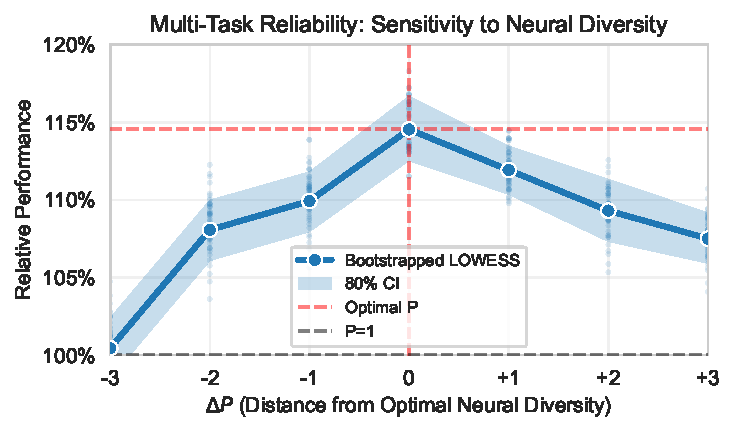
\includegraphics[width=0.85\textwidth]{assets/figure1_optimal_diversity.pdf}
  \end{center}
  \caption{
    \textbf{Maximizing reliability requires an optimal amount of neural diversity.} We vary parallel
    decorrelated representations ($P \in \{1,2,4,8\}$) and measure performance across 6 hallucination
    benchmarks. The x-axis shows distance from the performance-maximizing $P_\star$: $\Delta P = P -
    P_\star$. Aggregating 182,850 evaluation points (LOWESS fit, 80\% bootstrap CI, 1000 bootstrap
    resamplings), the U-shaped curve shows performance improves rapidly with neural diversity, peaking at a
    specific optimum and then degrading slowly with excessive parallelism.
  }
  \label{fig:optimaldiv}
\end{figure}

\section{Introduction}
Despite scaling to trillions of parameters, language models hallucinate persistently \citep{lin2021truthfulqa}.
This reliability crisis is acute for small language models (SLMs) --- increasingly favored for edge deployment
\citep{chen2024edge} --- whose compressed representations make them especially vulnerable to hallucinations, with
even well-resourced efforts like GPT-OSS 20B exhibiting 91\% hallucination rates on factual benchmarks
\citep{openai2025gptoss}.

Existing scaling methods --- parameters, inference-time compute, and parallel architectures like ParScale
\citep{chen2025parscale} --- predominantly target \emph{accuracy} (first-moment improvements in perplexity and
task performance). Yet \emph{reliability} (second-moment reduction in hallucinations and factual errors) remains
largely unaddressed. While ParScale achieves $O(\log P)$ performance gains with better memory and latency,
it provides no explicit mechanism for reducing hallucinations. Without explicit regularization,
\emph{representational collapse} \citep{jing2022dimensional} drives parallel streams toward identical features,
leaving reliability gains unrealized despite added computational resources.

Drawing from portfolio theory, we propose that decorrelated representations reduce hallucination risk just as
uncorrelated assets reduce financial risk. When streams are perfectly correlated ($\rho=1$), parallelism provides
no benefit; when decorrelated ($\rho \to 0$), signal-to-noise improves by $\sqrt{P}$.

% FIXME: Re-prove scaling patterns. Too much detail.
We formalize this through a \textbf{neural diversity framework} proving hallucination probability is bounded by
cross-stream correlation: $\mathbb{P}(\text{hallucination}) \leq f(\sigma^2((1-\rho)/P + \rho), \mu^2)$. This
reveals why existing scaling approaches don't address reliability and how explicit decorrelation provides a
mechanism to reduce hallucinations at fixed parameter budgets.

To validate this, we introduce \textbf{ND-LoRA}, combining independent LoRA adapters with Barlow Twins
regularization \citep{zbontar2021barlow}. Despite adding only 0.004\% more computation, ND-LoRA reduces
hallucinations by up to 25.6\% (14.6\% avg.) while preserving general performance.

Our experiments establish: (1) neural diversity causally reduces hallucination probability; (2) there is an
optimal amount of neural diversity and that optimal amount is task-dependent; and (3) the relationship
between neural diversity and hallucination probability is theoretically provable.

Neural diversity represents a third scaling axis beyond parameters and data. While traditional scaling asks
``how big?" and data scaling ``how much?", diversity scaling asks ``how different?" --- crucial for achieving
reliability without massive computational investment.

Our contributions are:
\begin{itemize}
  \item \textbf{Theory}: The first principled connection between neural spectral diversity and hallucination
    probability that matches empirically observed hallucination rates
  \item \textbf{Method}: ND-LoRA, a parameter-efficient demonstration achieving up to 25.6\% hallucination reduction
    and maintaining general-purpose accuracy at 1.00004$\times$ training cost
  \item \textbf{Analysis}: Evidence of the concavity of $P$ in industry-standard benchmarks and the presence
    of task-dependent optimal $P$ revealing when neural diversity helps most (and hurts)
  \item \textbf{Framework}: A general principle for parallel architectures --- that maintaining decorrelation is as
    important as adding capacity --- with implications beyond hallucination mitigation
\end{itemize}

\section{A Theory of Neural Diversity}
Why don't existing scaling methods improve reliability? Without explicit diversity mechanisms, gradient descent
drives parallel streams toward similar representations through \emph{representational collapse}
\citep{jing2022dimensional}, leaving reliability gains unrealized. We establish the first rigorous
connection between architectural diversity and hallucination probability, proving that decorrelated streams
reduce hallucinations and providing mathematical foundations for ND-LoRA.

\subsection{Preliminaries}
We develop a framework connecting parallel neural computation to hallucination probability. Consider a language
model processing input $x$ to produce an output (e.g., answer to a question, summary of a document). We say the
model \emph{hallucinates} when it generates content unsupported by its input or training knowledge --- for instance,
fabricating facts, misattributing quotes, or creating non-existent references.

Our architecture employs $P$ parallel computational pathways called \emph{streams}, each processing the same input
through the same model but in perturbed ways. Each stream $i$ produces a scalar \emph{margin} $m_i \equiv
m_i(x)$ representing its confidence: positive margins indicate the stream believes the output is
correct, while negative margins signal likely errors. These streams are combined through a weighted average
to produce the final prediction:
\begin{equation}
  M \;\triangleq\; \frac{1}{P}\sum_{i=1}^P m_i.
\end{equation}

We model each stream with mean confidence $\E[m_i]=\mu$ (with $\mu>0$ for correct outputs), per-stream variance
$\Var(m_i)=\sigma^2$, and pairwise correlations $\rho_{ij}=\mathrm{Corr}(m_i,m_j)$ measuring how similarly
streams behave. The \emph{average pairwise correlation} captures overall stream similarity:
\begin{equation}
  \rho \;\triangleq\; \frac{2}{P(P-1)}\sum_{1\le i<j\le P}\rho_{ij}.
\end{equation}
We define the hallucination event as $\HALL \equiv \{M\le 0\}$---when the aggregated margin crosses zero,
indicating the ensemble prediction is incorrect.

The key intuition is diversification: when streams are perfectly correlated ($\rho = 1$), they make identical
errors and averaging provides no benefit. When decorrelated ($\rho \to 0$), independent errors cancel out and
$M$ concentrates around its mean $\mu$, reducing hallucination probability as $P$ increases.

\subsection{Neural Diversity Bounds Hallucination}
We connect margin correlation to feature correlation through linearization: if predictions depend approximately
linearly on representations at a chosen design layer, then reducing feature correlation reduces margin correlation.

\textbf{Design-layer features and diversity.}
At a chosen \emph{design layer}, stream $i$ exposes a feature vector $z_i\in\mathbb{R}^d$. Let $\tilde z_i$
denote a whitened version (zero-mean, identity covariance within stream), and define the
\emph{cross-correlation} matrices $C_{ij}\triangleq \E[\tilde z_i \tilde z_j^\top]$.

\begin{definition}[Neural Diversity Index]
  \label{def:diversity}
  The spectral diversity index is
  \begin{equation}
    \mathcal{D}_{\mathrm{spec}}
    \;=\; \frac{1}{P(P-1)}\sum_{i\ne j}\,\norm{C_{ij}}_2.
  \end{equation}
\end{definition}

Lower $\mathcal{D}_{\mathrm{spec}}$ indicates greater diversity: $\mathcal{D}_{\mathrm{spec}} = 0$ means perfectly
decorrelated streams, while $\mathcal{D}_{\mathrm{spec}} = 1$ means complete collapse.

We now connect stream correlation to hallucination probability through three steps: variance analysis,
linearization, and the main bound.

\begin{lemma}[Variance of Aggregated Margin]
  \label{lem:var-aggregate}
  Under the assumptions above,
  \begin{equation}
    \Var(M) \;=\; \sigma^2\!\left(\frac{1-\rho}{P}+\rho\right).
  \end{equation}
\end{lemma}

\paragraph{Proof sketch.}
Expand $\Var(M)$ via $\Var(\frac1P\sum m_i)$, use $\Var(m_i)=\sigma^2$ and $\Cov(m_i,m_j)=\rho\,\sigma^2$ for
$i\neq j$, then collect terms.

When $\rho = 0$, variance decreases as $\sigma^2/P$. When $\rho = 1$, variance stays at $\sigma^2$ regardless of $P$.

% \begin{proposition}[Hallucination Probability Upper Bound]
%   \label{prop:cantelli}
%   By Cantelli's inequality,
%   \[
%     \Prob(M\le 0)
%     \;\le\; \frac{\Var(M)}{\Var(M)+\mu^2}
%     \;=\; \frac{\sigma^2\left(\tfrac{1-\rho}{P}+\rho\right)}{\sigma^2\left(\tfrac{1-\rho}{P}+\rho\right)+\mu^2}.
%   \]
% \end{proposition}

% \paragraph{Proof sketch.}
% Apply Cantelli to $X=M$ with mean $\mu>0$, taking $t=\mu$; then substitute Lemma~\ref{lem:var-aggregate}.

% \begin{proof}
%   Cantelli's inequality states that for any real $X$ with mean $\E[X]=\mu$ and variance $v>0$,
%   \[
%     \Prob(X-\mu \le -t) \;\le\; \frac{v}{v+t^2}\qquad\text{for all }t>0.
%   \]
%   Set $X=M$ and $t=\mu>0$:
%   \[
%     \Prob(M \le 0) \;=\; \Prob(M-\mu \le -\mu) \;\le\; \frac{\Var(M)}{\Var(M)+\mu^2}.
%   \]
%   Now plug in Lemma~\ref{lem:var-aggregate}.
% \end{proof}

\begin{lemma}[Correlation Bound]
  \label{lem:corr-bound}
  Assume the margins are locally linear in whitened features,
  $m_i = v_i^\top \tilde z_i$, and let $\sigma_i^2\triangleq \Var(m_i)$.
  Then for $i\neq j$,
  \begin{equation}
    \rho_{ij}
    \;=\; \frac{\Cov(m_i,m_j)}{\sigma_i\sigma_j}
    \;\le\; \kappa_{ij}\,\norm{C_{ij}}_2,
    \qquad
    \kappa_{ij}\;\triangleq\; \frac{\norm{v_i}\,\norm{v_j}}{\sigma_i\sigma_j}.
  \end{equation}
\end{lemma}

\paragraph{Proof sketch.}
Compute $\Cov(m_i,m_j)=v_i^\top C_{ij}v_j$ and bound by the spectral norm: $|v_i^\top C_{ij}v_j|\le
\norm{v_i}\,\norm{C_{ij}}_2\,\norm{v_j}$. Divide by $\sigma_i\sigma_j$.

Margin correlation $\rho_{ij}$ is controlled by feature correlation $\|C_{ij}\|_2$. We now have a direct path
from $\mathcal{D}_{\mathrm{spec}}$ to hallucination probability.

\begin{theorem}[Hallucination Probability Bound with Diversity]
  \label{thm:halluc-with-diversity}
  The hallucination probability satisfies
  \begin{equation}
    \Prob(\HALL)
    \;\le\;
    \frac{\sigma^2\left(\tfrac{1 - \bar{\kappa}\,\mathcal{D}_{\mathrm{spec}}}{P}
    + \bar{\kappa}\,\mathcal{D}_{\mathrm{spec}}\right)}
    {\sigma^2\left(\tfrac{1 - \bar{\kappa}\,\mathcal{D}_{\mathrm{spec}}}{P}
    + \bar{\kappa}\,\mathcal{D}_{\mathrm{spec}}\right) + \mu^2}
    \;+\; h_0,
  \end{equation}
  where $\bar{\kappa}$ is the average correlation scaling factor and $0\le h_0\le 1$ is a constant accounting
  for approximation error.
\end{theorem}

\paragraph{Proof sketch.}
By \autoref{lem:var-aggregate}, $\Var(M)$ is increasing in $\rho$ for $P>1$. $\bar\rho \le
\bar\kappa\,\mathcal{D}_{\mathrm{spec}}$, hence $\Var(M) \le
\sigma^2\!\big(\tfrac{1-\bar\kappa \mathcal{D}_{\mathrm{spec}}}{P}+\bar\kappa
\mathcal{D}_{\mathrm{spec}}\big)$. Plug this variance bound into Cantelli's bound. If the linear/whitening
conditions fail on a set of probability $h_0$, upper bound that set trivially by
1 and add $h_0$.

This gets us the first half of our theoretical result: Lower $\mathcal{D}_{\mathrm{spec}}$ reduces
hallucination probability and, additionally, the benefit scales with $P$.

\subsection{Scaling Behavior}
Next, we demonstrate that under common circumstances, the hallucination bound follows a U-shaped
curve --- initially decreasing with higher $P$, but starts increasing eventually. Consider the case where the
correlation itself increases with $P$, say, due to optimizer constraints:

\begin{theorem}[``U-shape'' of the Hallucination Bound under Rising Correlation]
  \label{thm:u-shape}
  Suppose the average correlation increases with $P$ as
  $\rho(P)=\rho_0+\beta(P-1)^\gamma$ with $\beta>0$ and $\gamma>0$,
  and consider the Cantelli bound:
  \begin{equation}
    \mathcal{B}(P)
    \;\triangleq\;
    \frac{\sigma^2\left(\tfrac{1-\rho(P)}{P}+\rho(P)\right)}
    {\sigma^2\left(\tfrac{1-\rho(P)}{P}+\rho(P)\right) + \mu^2}.
  \end{equation}
  Then $\mathcal{B}(P)$ is \emph{decreasing} for $P$ near $1$ and \emph{increasing} for $P$ sufficiently large.
  Moreover, if $\gamma\ge 1$ (so $\rho''(P)\ge 0$), $\mathcal{B}(P)$ is convex on $(1,\infty)$ and thus has a
  \emph{unique} minimizer $P_{\star}>1$.
\end{theorem}

\paragraph{Proof sketch.}
Work with the unnormalized variance factor
$g(P)=\tfrac{1-\rho(P)}{P}+\rho(P)$.
Differentiate:
$g'(P)=\rho'(P)\big(1-\tfrac{1}{P}\big) - \tfrac{1-\rho(P)}{P^2}$.
At $P\downarrow 1$, the first term vanishes while the second is negative, so $g'(P)<0$.
As $P\to\infty$, $\rho'(P)>0$ dominates the $O(P^{-2})$ negative term, so $g'(P)>0$ eventually.
If $\gamma\ge 1$, then $g''(P)\ge 0$, giving a unique minimizer.
Since $\mathcal{B}(P)$ is an increasing function of $g(P)$, the same qualitative behavior holds for $\mathcal{B}(P)$.

All together, Theorems \ref{thm:halluc-with-diversity} and \ref{thm:u-shape} show that there exists an optimal
$P_{\star}$ that minimizes hallucinations. Next, we show how to construct an architecture and training
protocol to find $P_{\star}$.

\section{ND-LoRA: A Practical Demonstration}
% FIXME: Add concrete example for intuition, e.g. A lot of Bens were born in 2012, when was Ben Franklin
% born? That is, can't correct hallucinations due to first moment (things LLM learned as an a priori mode),
% but can help correct noise and/or distractions.
\begin{figure}[ht]
  \begin{center}
    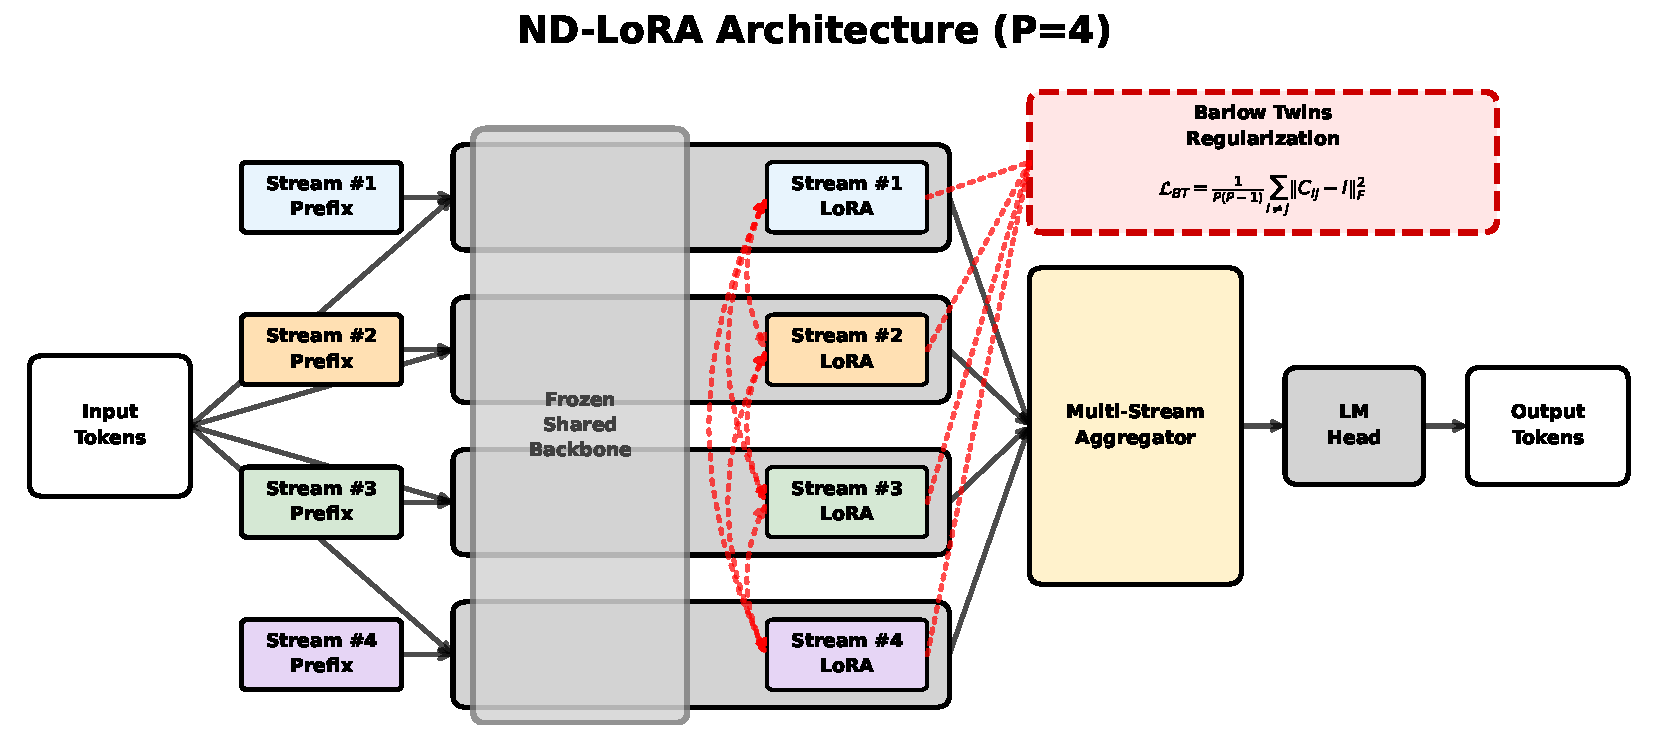
\includegraphics[width=1\textwidth]{assets/figure2_diagram.pdf}
  \end{center}
  \caption{
    \textbf{ND-LoRA schematic for $P=4$ parallel streams.} Each stream receives independent LoRA adapters
    and learnable prefix tokens. The aggregator combines stream outputs with learnable weights, while
    Barlow Twins regularization incentivizes decorrelation between stream outputs.
  }
  \label{fig:diagram}
\end{figure}

We introduce ND-LoRA (Neural Diversity Low-Rank Adaptation), a parameter-efficient method that demonstrates our
theoretical framework for neural diversity regularization. ND-LoRA extends the ParScale architecture with
stream-aware LoRA adapters and explicit decorrelation objectives.

\subsection{Architecture}
Our implementation builds on ParScale with $P$ parallel computation streams. Each stream $i \in \{1,
\ldots, P\}$ uses 48 learnable prefix tokens prepended to the input sequence that flow through all layers
via the attention mechanism, along with stream-specific LoRA adapters applied at each layer:
\begin{equation}
  h_i^{(\ell)} = \text{Layer}^{(\ell)}(h_i^{(\ell-1)} + B_i^{(\ell)} A_i^{(\ell)} h_i^{(\ell-1)})
\end{equation}
where $B_i^{(\ell)} \in \mathbb{R}^{d \times r}$, $A_i^{(\ell)} \in \mathbb{R}^{r \times d}$ are stream-specific
LoRA matrices with rank $r$. The final output combines streams through a learned aggregator:
\begin{equation}
  y = \text{LM\_Head}\left(\sum_{i=1}^P \alpha_i \cdot h_i^{(L)}\right)
\end{equation}
where $\alpha_i = (1-\varepsilon) \cdot \text{softmax}(\text{MLP}([h_1^{(L)}, \ldots, h_P^{(L)}]))_i +
\varepsilon/P$ are dynamic weights with
label smoothing ($\varepsilon = 0.1$) computed from the concatenated stream representations.
This prevents attention collapse by ensuring minimum weight $\varepsilon/P$ for each stream.

This architecture enables stream specialization while maintaining parameter efficiency. For $P=2$ streams
with rank-16 LoRA, we use approximately 29K trainable parameters per layer, comparable to a single rank-32
LoRA but with fundamentally different representational capabilities.

\subsection{Barlow Twins Regularization}
To encourage neural diversity, we apply Barlow Twins regularization at a pre-specified design layer $\ell^*$. Let
$z_i^{(\ell^*)} \in \mathbb{R}^{B \times T \times d}$ denote the hidden representations of stream $i$ at the
design layer. We first apply batch normalization and mean-centering to obtain whitened features $\tilde{z}_i$.

The cross-correlation matrix between streams $i$ and $j$ is:
\begin{equation}
  C_{ij} = \frac{1}{BT} \sum_{b,t} \tilde{z}_{i,bt} \tilde{z}_{j,bt}^\top \in \mathbb{R}^{d \times d}
\end{equation}
Our Barlow Twins loss promotes decorrelation by penalizing off-diagonal correlations:
\begin{equation}
  \mathcal{L}_{BT} = \frac{1}{P(P-1)} \sum_{i \neq j} \|C_{ij} - I\|_F^2
\end{equation}
The standard formulation scales quadratically with $P$, creating $\binom{P}{2}$ optimization dependencies
that inhibit convergence. To address this scalability challenge, we implement a RandK variant that
samples stream pairs stochastically:
\begin{equation}
  \mathcal{L}_{BT} = \mathbb{E}_{(i,j) \sim \text{MultN}(C_i)} \|C_{ij} - I\|_F^2
\end{equation}
where $C_i$ induces a multinomial distribution over stream pairs. This reduces complexity from $O(P^2)$ to
$O(PK)$ where $K$ is the number of sampled pairs, enabling efficient scaling to larger $P$.

The total training objective combines cross-entropy and decorrelation terms:
\begin{equation}
  \mathcal{L} = \mathcal{L}_{CE} + \lambda_{BT} \mathcal{L}_{BT}
\end{equation}

\section{Experimental Validation}
\subsection{Experimental Setup}
We validate our theoretical framework through systematic hallucination reduction experiments using neural
diversity regularization with parameter- and data-matched comparisons.

\textbf{Model and Architecture.} We use Qwen2.5-0.5B (896 hidden dimensions, 24 layers) with ND-LoRA
across $P \in \{1, 2, 4, 8\}$ parallel streams applied to QKV self-attention modules and a design layer of
20 for de-correlation loss. Each stream uses independent rank-16 LoRA adapters and 48 prefix tokens, totaling
5-20M trainable parameters with 494M backbone frozen. Baseline methods use higher-rank LoRA (R32-R128) for
parameter matching.

\textbf{Training Protocol.} Models train on 20M tokens from The Pile (8 random shards, fixed seeds). We use
1024-token sequences, AdamW optimization (peak lr 3e-4, cosine decay, 2\% warmup), batch size 64, bfloat16
precision, design layer 16. Training completes in ~5K steps (~30 minutes on A100).

\textbf{Evaluation Benchmarks.} We evaluate across: (1) \emph{Hallucination-sensitive}: TruthfulQA
\citep{lin2021truthfulqa}, HaluEval \citep{li2023halueval}, MemoTrap \citep{mckenzie2023inverse}; (2)
\emph{Knowledge-intensive}: Natural Questions \citep{kwiatkowski2019natural}, TriviaQA
\citep{joshi2017triviaqa}, PopQA \citep{mallen2023trust}; (3) \emph{General capability}: Wikitext BPB
\citep{merity2017pointer}, Winogrande \citep{sakaguchi2020winogrande}. This tests if neural diversity
improves reliability without sacrificing general performance.

\textbf{Statistical Methodology.} We evaluate significance using McNemar's test for binary classification
tasks and two-tailed bootstrap tests with 10,000 samples for other tasks. Improvements marked with * are
significant at $p < 0.05$.

\subsection{Key Results}
\autoref{tab:relacc} demonstrates ND-LoRA achieves substantial improvements on hallucination-sensitive
benchmarks while maintaining competitive general performance. ND-LoRA with $P=2$ streams achieves statistically
significant improvements on HaluEval-Summarization (0.481* vs 0.400, $p < 0.001$, 8.1\% absolute / 20.2\% relative),
TruthfulQA-MC2 (0.442* vs 0.403, $p = 0.030$, 3.9\% absolute / 9.5\% relative) and MemoTrap (0.666* vs 0.634, $p
< 0.001$, 3.2\% absolute / 5.1\% relative) vs parameter-matched Qwen, validating our theoretical prediction.

Although ND-LoRA's improvements specifically target reliability benchmarks, they preserve general
capabilities. Qwen slightly outperforms on Wikitext (0.784 vs 0.778) and Natural Questions
(0.055 vs. 0.065), but ND-LoRA wins on Winogrande (0.574). This task-selective pattern aligns with our
framework for non-monotone behaviors and task-dependent optimality.

Parameter efficiency is evident comparing ND-LoRA R16 ($P=2$) against Qwen2.5-0.5B LoRA R32. Despite lower-rank
adapters, ND-LoRA consistently outperforms the high-rank baseline on hallucination tasks, demonstrating that
architectural diversity provides more value at equal capacity. This shows representational diversity, not
parameter count, drives reliability gains in our experiment.

\begin{table}[t]
  \begin{center}
    \begin{tabular}{lcccccc}
      \multicolumn{1}{c}{\bf Model} &
      \multicolumn{1}{c}{\bf HaluEval} &
      \multicolumn{1}{c}{\bf MemoTrap} &
      \multicolumn{1}{c}{\bf TruthfulQA} &
      \multicolumn{1}{c}{\bf NQ} &
      \multicolumn{1}{c}{\bf Wikitext} &
      \multicolumn{1}{c}{\bf WG}
      \\ \hline \\[-0.75em]
      ND-LoRA R16 (P=2)        & \textbf{0.481*} & \textbf{0.666*} & \textbf{0.442*} & 0.055 & 0.784 & \textbf{0.574} \\
      ParScale R32 (P=2)       & 0.439 & 0.638 & 0.412 & 0.059 & 0.793 & 0.564 \\
      Qwen LoRA R32            & 0.400 & 0.634 & 0.403 & \textbf{0.065} & \textbf{0.778} & 0.572 \\
    \end{tabular}
  \end{center}
  \caption{
    \textbf{Even at $P=2$ streams, ND-LoRA achieves up to 20.2\% relative hallucination reduction vs.
    parameter-matched baseline.} Across hallucination benchmarks, ND-LoRA shows statistically
    significant improvements (HaluEval-Summarization +20.2\%*, MemoTrap +5.1\%*, TruthfulQA-MC2 +9.5\%*)
    while maintaining competitive Winogrande, NQ, and Wikitext general-purpose capabilities. Baselines use higher
    LoRA ranks for parameter parity. * indicates $p < 0.05$.
  }
  \label{tab:relacc}
\end{table}

\begin{figure}[t]
  \begin{center}
    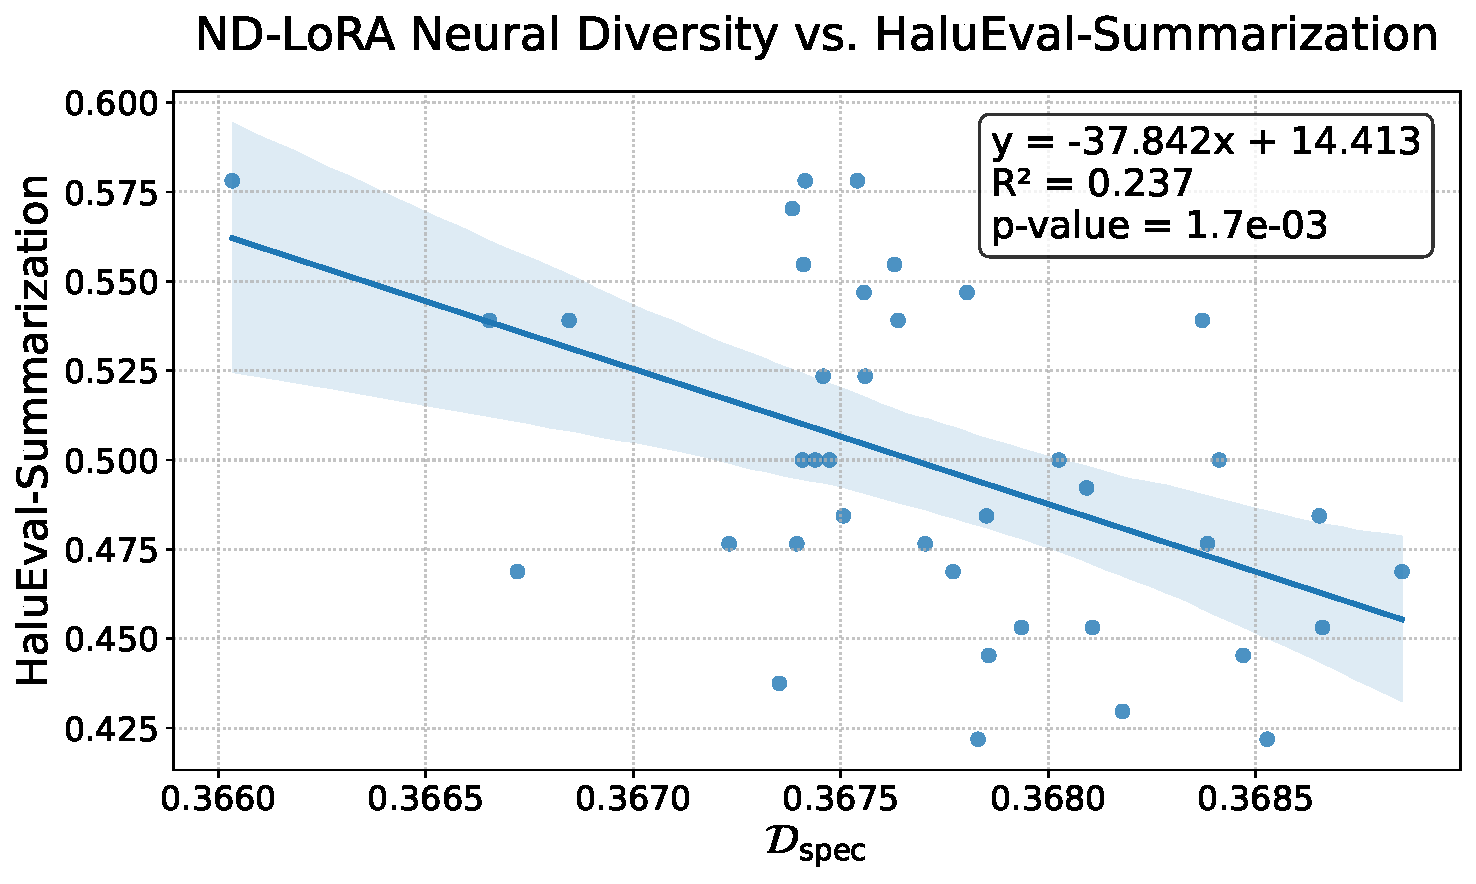
\includegraphics[width=0.85\textwidth]{assets/figure3_correlational_intuition.pdf}
  \end{center}
  \caption{
    \textbf{Reliability improves as neural diversity increases (lower $\mathcal{D}_{\text{spec}}$).} Specifically,
    spectral diversity ($\mathcal{D}_{\text{spec}}$) is negatively correlated with HaluEval-Summarization
    performance (slope=-37.842, R²=0.237, p=0.002), consistent with $\mathbb{P}(\text{H}) \propto
    \mathcal{D}_{\text{spec}}$ in \autoref{thm:halluc-with-diversity}.
  }
  \label{fig:correlational}
\end{figure}

These findings establish neural diversity as a practical reliability mechanism. Consistent improvements
across hallucination benchmarks with preserved general performance suggest ND-LoRA addresses fundamental
reliability challenges rather than metric-specific optimization. \autoref{fig:correlational} demonstrates
strong empirical correlation between neural diversity and performance, building intuition for the causal
relationship established in Section 5.

\subsection{Scaling Analysis}
Our theoretical framework predicts U-shaped scaling curves where hallucination probability initially
decreases with $P$ but increases as correlation rises without diversity regularization.
\autoref{fig:optimaldiv} empirically validates this across tasks, revealing a critical insight: maximizing
reliability requires an \emph{optimal amount} of neural diversity --- more diversity is not always better.

\subsection{Task-Dependent Optimality}
\begin{table}[t]
  \begin{center}
    \begin{tabular}{ll|cccc}
      \multicolumn{1}{c}{\bf Category} &
      \multicolumn{1}{c}{\bf Task} &
      \multicolumn{1}{c}{\bf Best $P$} &
      \multicolumn{1}{c}{\bf Best Score} &
      \multicolumn{1}{c}{\bf ${\Delta}$\% Score} &
      \multicolumn{1}{c}{\bf Sig.}
      \\ \hline \\[-0.75em]
      \multirow{6}{*}{Hallucination}
      & HaluEval (Dialog)    & 4 & 0.516 & +12.8\% & *** \\
      & HaluEval (QA)        & 4 & 0.451 & +23.4\% & *** \\
      & HaluEval (Summ)      & 4 & 0.502 & +25.6\% & *** \\
      & MemoTrap v2          & 8 & 0.689 & +8.8\%  & *** \\
      & TruthfulQA (MC1)     & 2 & 0.269 & +7.3\%  & \\
      & TruthfulQA (MC2)     & 2 & 0.442 & +9.5\%  & * \\
      \hline \\[-0.75em]
      \multirow{4}{*}{Knowledge}
      & NQ (8-shot)          & 1 & 0.066 & --      & \\
      & NQ-swap              & 8 & 0.554 & +0.8\%  & \\
      & PopQA                & 1 & 0.111 & --      & \\
      & TriviaQA (8-shot)    & 1 & 0.192 & --      & \\
    \end{tabular}
  \end{center}
  \caption{\textbf{The optimal amount of neural diversity varies by task.} Hallucination tasks show large gains
    with optimal $P \in \{2,4,8\}$ (up to +25.6\%), while knowledge tasks mostly peak at $P=1$. Even among
    hallucination tasks, optimal $P$ differs: HaluEval variants peak at $P=4$, TruthfulQA at $P=2$, MemoTrap at
    $P=8$. Each row shows the performance peak (best $P$), best score, relative increase vs. $P=1$ baseline, and
  statistical significance (*** for $p < 0.001$, * for $p < 0.05$).}
  \label{tab:taskdiv}
\end{table}

Further, the optimal diversity is task-dependent. \autoref{tab:taskdiv} reveals striking task-dependent
sensitivity patterns relative to the $P=1$ baseline. Hallucination-focused tasks show the largest
gains: HaluEval Summarization achieves +25.6\% relative improvement at $P=4$, HaluEval QA shows +23.4\% at $P=4$,
and TruthfulQA MC2 shows +9.5\% at $P=2$ while MemoTrap benefits from higher diversity ($P=8$, +8.8\%).
Notably, knowledge-intensive tasks like PopQA, TriviaQA and NQ show no improvement over baseline, which is
expected as ND-LoRA does not add new sources of knowledge or try to improve recall of existing knowledge.
This heterogeneity demonstrates that different tasks require different amounts of neural diversity to
maximize reliability, with hallucination-focused tasks generally benefiting most from decorrelated representations.

\section{Mechanistic Analysis}
\subsection{Neural Diversity as the Causal Mediator}
\label{sec:causality}
To establish causality beyond correlation, we perform artificial corruption interventions that directly
manipulate cross-stream similarity.

\textbf{Experiment Design.}
Starting with a pre-trained ND-LoRA $P=4$ model, we inject a corruption hook at the RMSNorm layer that
randomly substitutes the hidden state at randomly-chosen positions in a given stream from another stream , reducing
$\mathcal{D}_{\text{spec}}$ while preserving activation magnitudes. We evaluate on a matched basis: each
corrupted evaluation is paired with an uncorrupted baseline using identical samples and resampling indices.
Across 4 sub-experiments with different random seeds, we collect N=128 paired samples per task. This paired
design maximizes statistical power by controlling sample-level variance, analyzed via paired t-tests with
Fisher meta-analysis.

\textbf{Results.}
\autoref{tab:causality} provides statistically robust evidence that neural diversity causally affects
performance. All three tasks show highly significant accuracy drops ($p < 0.001$) when stream-level
substitution reduces diversity ($\Delta\mathcal{D}_{\text{spec}} \approx 0.025$). While effect sizes are
modest (0.3\% to 0.7\% score reduction) --- likely because artificial stream substitution creates
out-of-distribution corruption patterns --- the statistical significance establishes causality beyond
correlational association.

\begin{table}[t]
  \centering
  \begin{tabular}{l|ccccccc}
    \textbf{Task} & \textbf{$\Delta\mathcal{D}_{\text{spec}}$} & \textbf{$\Delta$ Score} & \textbf{SE} &
    \textbf{d} & \textbf{p-value} & \textbf{Sig.} & \textbf{N} \\
    \hline
    HaluEval-Summ & 0.024 & -0.005 & 0.010 & 0.007 & $1.6 \times 10^{-5}$ & *** & 512 \\
    MemoTrap v2 & 0.031 & -0.003 & 0.010 & 0.000 & $8.2 \times 10^{-5}$ & *** & 512 \\
    TruthfulQA-MC2 & 0.025 & -0.007 & 0.009 & 0.018 & $3.3 \times 10^{-7}$ & *** & 512 \\
  \end{tabular}
  \caption{
    \textbf{Artificial corruption of neural diversity establishes statistical causality.} Reducing neural diversity
    ($\Delta\mathcal{D}_{\text{spec}} > 0$) causes accuracy drops across tasks with high statistical
    significance ($p < 0.001$) via paired t-tests with Fisher meta-analysis (N=4 sub-experiments × 128 samples each).
  }
  \label{tab:causality}
\end{table}

\subsection{Ablations}
To isolate the contributions of ND-LoRA, we systematically ablate ND-LoRA components at fixed $P=4$ streams.
All variants maintain parameter parity through LoRA rank adjustments, enabling fair comparison. We measure
run-time spectral diversity ($\mathcal{D}_{\text{spec}}$) at the aggregation layer using evaluation samples,
quantifying actual cross-stream correlation during inference.

\autoref{tab:ablations} reveals a super-linear combination: independent LoRA (+2.9\%) and Barlow Twins
(+1.4\%) sum to 4.3\% but achieve 4.9\% when combined (Stream LoRA-BT) --- a 14\% bonus. Targeting KVQ
attention amplifies this further by 2.6$\times$ to +12.8\% (ND-LoRA at fixed $P=4$; maximum gains reach
14.6\% when optimizing $P$ per-task, see \autoref{tab:taskdiv}). Neither component alone
suffices: ParScale's near-complete collapse ($\mathcal{D}_{\text{spec}} = 0.999$) yields only +0.5\%, while
Stream LoRA without regularization achieves +2.9\%, both less than a quarter of ND-LoRA's final impact. This
establishes that both architectural capacity and explicit regularization are necessary for full impact.

Counterintuitively, ND-LoRA achieves best performance (+12.8\%) with \emph{higher} $\mathcal{D}_{\text{spec}}
= 0.376$ than Stream LoRA-BT's 0.140 (lowest across all variants). This reveals that strategic localization
to representational bottlenecks matters more than maximizing global decorrelation: focusing LoRA and Barlow
Twins on KVQ attention modules --- where information flow is controlled --- provides 2.6$\times$ amplification
over applying them uniformly across all layers. Consistent with \autoref{tab:taskdiv}, this demonstrates
neural diversity is a task-dependent resource requiring strategic allocation to critical computational
pathways rather than uniform application.

\subsection{Computational Considerations}
ND-LoRA achieves substantial reliability gains with negligible overhead (1.00004$\times$ training,
1.1$\times$ inference). Three factors drive efficiency: (a) 20M token training amortizes to ~0.004\% of 1T
pretraining; (b) frozen 494M backbone makes gradients through 1.3M parameters nearly free; (c) ND-LoRA and
ParScale require identical FLOPs during inference, simply loading different LoRA adapters per stream. Unlike $P$-model
ensembles with $P\times$ training cost, ND-LoRA achieves neural diversity within a single architecture.
See Appendix \ref{sec:cost_analysis} for details.
% FIXME: Add 4xSLM ensemble benchmark.

\begin{table}[t]
  \small
  \begin{center}
    \begin{tabular}{l|cccc|ccccc}
      \multicolumn{1}{c}{\bf Variant} &
      \multicolumn{1}{c}{\bf Streams} &
      \multicolumn{1}{c}{\bf LoRA} &
      \multicolumn{1}{c}{\bf Regul.} &
      \multicolumn{1}{c}{\bf Target} &
      \multicolumn{1}{c}{\bf $\mathcal{D}_{\text{spec}}$} &
      \multicolumn{1}{c}{\bf $\overline{\Delta}$\% Score} &
      \multicolumn{1}{c}{\bf $\Delta$ Cost}
      \\ \hline \\[-0.75em]
      Standard       & 1   & Single & D      & All & --              & 0.0\%  & ~~~~~~~~\textbf{1.0x} / \textbf{1.0x} \\
      ParScale       & $P$ & Single & D      & All & 0.9991          & +0.5\%           & 1.00003x / 1.1x \\
      ParScale-BT    & $P$ & Single & D + BT & All & 0.9988          & +1.4\%           & 1.00003x / 1.1x \\
      Stream LoRA    & $P$ & Stream & D      & All & 0.2678          & +2.9\%           & 1.00003x / 1.1x \\
      Stream LoRA-BT & $P$ & Stream & D + BT & All & \textbf{0.1400} & +4.9\%           & 1.00004x / 1.1x \\
      ND-LoRA        & $P$ & Stream & D + BT & KVQ & 0.3755          & \textbf{+12.8\%} & 1.00004x / 1.1x \\
    \end{tabular}
  \end{center}
  \caption{
    \textbf{Ablations reveal super-linear combination of impact.} Stream LoRA (+2.9\%) and Barlow
    Twins (+1.4\%) combine super-linearly (+4.9\%), and focusing on KVQ attention amplifies to +12.8\%.
    {\em LoRA}: single shared vs. $P$ stream-aware adapters.
    {\em Regularization}: Dropout vs. Barlow Twins.
    {\em Target}: All layers vs. KVQ attention only.
    {\em $\mathcal{D}_{\text{spec}}$}: spectral diversity (lower better).
    {\em $\overline{\Delta}$\% Score}: avg. change (hallucination benchmarks).
  }
  \label{tab:ablations}
\end{table}

\section{Related Work}
\textbf{Hallucination in Language Models.}
Hallucinations represent a fundamental challenge in language model deployment \citep{huang2024survey,
tonmoy2024comprehensive},
proven mathematically inevitable in computable models \citep{xu2024inevitable, kalai2024calibrated}, with
particular severity in smaller models \citep{lin2021truthfulqa, li2023halueval}. Mechanistic investigations
reveal hallucinations arise from internal representation failures \citep{yu2024mechanistic, ferrando2025knowledge}.
Current mitigation strategies---retrieval augmentation \citep{niu2024ragtruth}, specialized decoding
\citep{li2023contrastive, manakul2023selfcheck, wei2024longform}, and constitutional training
\citep{bai2022constitutional}---address only specific aspects. MoE-LLaVA improves by 1.1\% on POPE but requires
$8\times$ parameters \citep{zhang2024moellava}. Our work achieves hallucination reduction through neural diversity
within a single architecture at fixed parameter budgets.

\textbf{Parallel Architectures and Scaling Laws.}
Parallel scaling offers a third axis beyond parameters and data \citep{chen2025parscale, kaplan2020scaling}.
ParScale achieves $O(\log P)$ gains with 22× less memory and 6× less latency \citep{chen2025parscale}, while
inference-optimal scaling laws favor smaller models with more data \citep{sardana2024beyond} and MoE achieves
1000× capacity through conditional computation \citep{shazeer2017sparsely}. However, these approaches target
accuracy rather than reliability. We show parallel scaling reduces hallucinations through explicit neural diversity.

\textbf{Diversity in Neural Networks.}
Deep ensembles provide improved accuracy and uncertainty estimates \citep{lakshminarayanan2017deep}, with
power-law scaling showing ~2\% gains \citep{lobacheva2020power} and PAC-Bayesian analysis proving error decreases
with $\sqrt{\text{diversity}}$ \citep{ortega2022diversity}. LLM ensembles achieve 2.2\% absolute MMLU improvements
\citep{tekin2024llmtopla}, while negative correlation learning demonstrates diversity must be actively encouraged
\citep{liu1999ensemble}. However, prior work targets general accuracy and requires multiple models. Our method
achieves substantially larger gains (8.1\% absolute / 25.6\% relative on hallucination benchmarks) at lower cost
(1.00004$\times$ vs. $P\times$ training) within a single architecture.

\textbf{Redundancy Reduction and Self-Supervised Learning.}
Self-supervised methods provide differentiable diversity mechanisms. Barlow Twins prevents collapse through
dimension decorrelation \citep{zbontar2021barlow}, VICReg decomposes into variance, invariance, and covariance
terms \citep{bardes2022vicreg}, and understanding dimensional collapse \citep{jing2022dimensional} reveals why
explicit decorrelation is necessary. We adapt these principles for hallucination reduction beyond visual learning.

\textbf{Parameter-Efficient Fine-Tuning.}
PEFT methods enable distinct streams under fixed budgets. LoRA reduces parameters by 10,000× with multiple
adapters inducing specialization \citep{hu2022lora, wang2023loraensemble}, prefix-tuning uses 0.1\% of parameters
\citep{li2021prefix}, and BitFit shows minimal differences enable specialization when regularized
\citep{benzaken2022bitfit}. BatchEnsemble and LoRA-Ensemble achieve diversity through clever parameterization
\citep{wen2020batchensemble, muhlematter2024loraensemble}, providing our technical foundation.

\textbf{Inference-Time Scaling and Aggregation.}
Self-consistency improves reasoning by 17.9\% through diverse sampling \citep{wang2022selfconsistency}, though
resampling has limitations with imperfect verifiers \citep{stroebl2024inference}. Confidence-based weighting
reduces required paths by 40\% \citep{taubenfeld2025confidence}, while contrastive decoding and classifier-free
guidance achieve improvements equivalent to parameter doubling \citep{li2023contrastive, sanchez2023cfg}. Unlike
post-hoc aggregation requiring multiple forward passes, our training-time parallelism learns coordinated streams.

\textbf{Theoretical Foundations.}
PAC-Bayesian bounds show minimax-optimal rates connecting diversity to generalization
\citep{steffen2024misclassification, biggs2022margins, ortega2022diversity}, while concentration inequalities
demonstrate that reducing predictor correlation tightens tail bounds on error events \citep{alquier2024userfriendly}.
This supports our approach of explicitly regularizing cross-stream correlation for factual reliability.

\section{Discussion}
Neural diversity establishes a principled framework bridging portfolio theory and deep learning to develop
models that are architecturally robust to noise. Our work provides both theoretical grounding --- proving
hallucination probability is bounded by cross-stream correlation --- and empirical validation through
ND-LoRA's 25.6\% hallucination reduction at negligible computational cost. The framework reveals why existing
scaling approaches target accuracy over reliability and how explicit decorrelation through neural diversity
provides a mechanism to reduce hallucinations at fixed parameter budgets, introducing a third scaling axis
orthogonal to parameters and data. Unlike traditional ensemble methods \citep{lakshminarayanan2017deep},
which require multiple separate models, our approach achieves diversity benefits within a single architecture.

At the same time, our demonstration has limitations. Computational constraints restricted experiments
to 0.5B models; larger-scale production-ready implementations are part of planned future work. Benchmark
scope focuses on English hallucination and knowledge tasks, with some tasks showing no benefit from increased
neural diversity, highlighting task-dependent efficacy that requires further investigation. Finally, while
our theoretical framework predicts non-monotonicity, it doesn't provide a satisfying explanation of why
different tasks have different optimality points.

As language models become critical infrastructure, reliability techniques that avoid massive resource investment
become essential. While hallucinations may be mathematically inevitable \citep{kalai2024calibrated}, neural diversity
demonstrates they can be systematically reduced through architectural design. Our results show reliable AI may
emerge from thoughtfully designed architectures rather than brute-force scaling alone, opening new avenues for
efficient, trustworthy language models.

\section*{Author Contributions}
Kushal Chakrabarti led the overall project design, core implementation of ND-LoRA, experimental design, and
paper writing. Nirmal Balachundhar contributed theoretical insights and implementation for novel neural
diversity techniques, experiment implementation and analysis, and paper writing.

\section*{Acknowledgments}
We thank the research community at South Park Commons for valuable discussions and feedback throughout this
project. We are grateful to Augustine Mavor-Parker, Bhav Ashok, David Sontag, Iman Modaressi, Jaclyn Lunger,
John Bohannon, Nelson Ray and Patrick Bozeman for their insightful comments on earlier drafts. This work was
supported by South Park Commons and Modal, who generously provided compute resources for our experiments.

\bibliography{main}
\bibliographystyle{iclr2026}

\appendix
\section{Appendix}
\subsection{Full Proofs}

\subsubsection{Proof of \autoref{lem:var-aggregate}}
\begin{proof}
  By bilinearity of covariance,
  \begin{align*}
    \Var(M)
    &= \Var\!\Big(\frac{1}{P}\sum_{i=1}^P m_i\Big)
    = \frac{1}{P^2}\Bigg(\sum_{i=1}^P \Var(m_i) \;+\; 2\sum_{1\le i<j\le P}\Cov(m_i,m_j)\Bigg)\\
    &= \frac{1}{P^2}\Big(P\,\sigma^2 \;+\; 2\cdot \tbinom{P}{2}\,\rho\,\sigma^2\Big)
    = \frac{1}{P^2}\Big(P\,\sigma^2 + P(P-1)\,\rho\,\sigma^2\Big)\\
    &= \sigma^2\!\left(\frac{1}{P} + \frac{P-1}{P}\,\rho\right)
    = \sigma^2\!\left(\frac{1-\rho}{P}+\rho\right).
  \end{align*}
\end{proof}

\subsubsection{Proof of \autoref{lem:corr-bound}}
\begin{proof}
  Since $m_i=v_i^\top \tilde z_i$ and $m_j=v_j^\top \tilde z_j$,
  \begin{equation}
    \Cov(m_i,m_j)
    = \E\big[ (v_i^\top \tilde z_i)(v_j^\top \tilde z_j) \big]
    = v_i^\top \E[\tilde z_i \tilde z_j^\top] v_j
    = v_i^\top C_{ij} v_j.
  \end{equation}
  By the definition of the spectral norm,
  \begin{equation}
    |\Cov(m_i,m_j)|
    = |v_i^\top C_{ij} v_j|
    \le \norm{v_i}\,\norm{C_{ij}}_2\,\norm{v_j}.
  \end{equation}
  Divide both sides by $\sigma_i\sigma_j$ to obtain
  \begin{equation}
    |\rho_{ij}| \le \frac{\norm{v_i}\,\norm{C_{ij}}_2\,\norm{v_j}}{\sigma_i\sigma_j}
    = \kappa_{ij}\,\norm{C_{ij}}_2.
  \end{equation}
  Since the right-hand side is nonnegative, this yields the stated upper bound on $\rho_{ij}$.
\end{proof}

\subsubsection{Proof of \autoref{thm:halluc-with-diversity}}
\begin{proof}
  Let $\rho_{ij}=\mathrm{Corr}(m_i,m_j)$ and
  $\bar\rho \triangleq \frac{2}{P(P-1)}\sum_{i<j}\rho_{ij}$.
  With common per-stream variance $\sigma^2$,
  \begin{align*}
    \Var(M)
    &= \Var\!\Big(\frac1P\sum_{i=1}^P m_i\Big)
    = \frac{1}{P^2}\Big(\sum_i \Var(m_i) \;+\; 2\sum_{i<j}\Cov(m_i,m_j)\Big) \\
    &= \frac{1}{P^2}\Big(P\sigma^2 + 2\textstyle\binom{P}{2}\sigma^2\,\bar\rho\Big)
    = \sigma^2\!\left(\frac{1}{P}+\frac{P-1}{P}\,\bar\rho\right)
    = \sigma^2\!\left(\frac{1-\bar\rho}{P}+\bar\rho\right).
  \end{align*}
  Next, by the linear feature model $m_i=v_i^\top \tilde z_i$ and the definition of
  $C_{ij}=\E[\tilde z_i \tilde z_j^\top]$,
  \begin{equation}
    \Cov(m_i,m_j)=v_i^\top C_{ij} v_j,
    \qquad
    |\Cov(m_i,m_j)| \le \|v_i\|\,\|C_{ij}\|_2\,\|v_j\|.
  \end{equation}
  Dividing by $\sigma_i\sigma_j$ gives
  \begin{equation}
    \rho_{ij}\;=\;\frac{\Cov(m_i,m_j)}{\sigma_i\sigma_j}
    \;\le\; \frac{\|v_i\|\,\|v_j\|}{\sigma_i\sigma_j}\, \|C_{ij}\|_2
    \;=\; \kappa_{ij}\,\|C_{ij}\|_2.
  \end{equation}
  Averaging over unordered pairs,
  \begin{align*}
    \bar\rho
    = \frac{2}{P(P-1)}\sum_{i<j}\rho_{ij}
    \;\le\; \frac{2}{P(P-1)}\sum_{i<j}\kappa_{ij}\,\|C_{ij}\|_2
    = \bar\kappa \cdot \frac{2}{P(P-1)}\sum_{i<j}\|C_{ij}\|_2
    = \bar\kappa\,\mathcal{D}_{\mathrm{spec}}.
  \end{align*}
  Because $\Var(M)$ is increasing in $\bar\rho$ for $P>1$,
  \begin{equation}
    \Var(M)
    \;\le\; \sigma^2\!\left(\frac{1-\bar\kappa\,\mathcal{D}_{\mathrm{spec}}}{P}
    + \bar\kappa\,\mathcal{D}_{\mathrm{spec}}\right).
  \end{equation}
  Applying Cantelli's inequality to $M$ with $\E[M]=\mu>0$ and $t=\mu$,
  \begin{equation}
    \mathbb{P}(M\le 0)
    = \mathbb{P}(M-\mu\le -\mu)
    \le \frac{\Var(M)}{\Var(M)+\mu^2}
    \le
    \frac{\sigma^2\left(\tfrac{1 - \bar{\kappa}\,\mathcal{D}_{\mathrm{spec}}}{P}
    + \bar{\kappa}\,\mathcal{D}_{\mathrm{spec}}\right)}
    {\sigma^2\left(\tfrac{1 - \bar{\kappa}\,\mathcal{D}_{\mathrm{spec}}}{P}
    + \bar{\kappa}\,\mathcal{D}_{\mathrm{spec}}\right) + \mu^2}.
  \end{equation}
  Finally, if assumptions (ii)–(iii) hold only on a ``good'' event $G$ with $\mathbb{P}(G)\ge 1-h_0$,
  then
  \begin{equation}
    \mathbb{P}(M\le 0)
    = \mathbb{P}(M\le 0\mid G)\,\mathbb{P}(G)
    + \mathbb{P}(M\le 0\mid G^{\mathrm c})\,\mathbb{P}(G^{\mathrm c})
    \le \mathbb{P}(M\le 0\mid G) + h_0,
  \end{equation}
  and the displayed fraction bounds $\mathbb{P}(M\le 0\mid G)$, yielding the stated result.
\end{proof}

\subsubsection{Proof of \autoref{thm:u-shape}}
\begin{proof}
  Let $g(P)\triangleq \tfrac{1-\rho(P)}{P}+\rho(P)$ so that $\mathcal{B}(P)$ is an increasing function of
  $g(P)$ (monotonicity in the numerator).
  Compute
  \begin{equation}
    g'(P)
    = \frac{d}{dP}\!\left(\frac{1-\rho(P)}{P}\right) + \rho'(P)
    = \Big(-\frac{\rho'(P)}{P} - \frac{1-\rho(P)}{P^2}\Big) + \rho'(P)
    = \rho'(P)\Big(1-\frac{1}{P}\Big) - \frac{1-\rho(P)}{P^2}.
  \end{equation}
  As $P\downarrow 1$, we have $1-\tfrac{1}{P}\to 0$ while $1-\rho(P)\to 1-\rho_0>0$, hence $g'(P)\to -(1-\rho_0)<0$.
  For large $P$, the negative term is $O(P^{-2})$, while $\rho'(P)=\beta\gamma(P-1)^{\gamma-1}>0$; thus for
  sufficiently large $P$, $g'(P)>0$.
  By continuity, there exists $P_\star>1$ with $g'(P_\star)=0$, implying that $g$ (and therefore
  $\mathcal{B}$) decreases for $P<P_\star$ and increases for $P>P_\star$.

  If $\gamma\ge 1$, then $\rho''(P)=\beta\gamma(\gamma-1)(P-1)^{\gamma-2}\ge 0$ and
  \begin{equation}
    g''(P)
    = \rho''(P)\Big(1-\frac{1}{P}\Big) + \frac{2\rho'(P)}{P^2} + \frac{2(1-\rho(P))}{P^3}\;\ge\;0
    \quad\text{for }P>1.
  \end{equation}
  Hence $g$ is convex on $(1,\infty)$ and has a unique minimizer; the same holds for $\mathcal{B}$, which is
  an increasing transform of $g$.
\end{proof}

\subsection{Training Cost and Latency Analysis}
\label{sec:cost_analysis}

This appendix provides a complete analysis of computational costs for ND-LoRA and baseline variants. Three key
insights enable negligible overhead: (1) fine-tuning on 20M tokens amortizes to less than 0.004\% of 1T pretraining,
(2) frozen backbone parameters make backward passes nearly free, and (3) inference uses identical FLOPs to
ParScale via dynamic LoRA swapping per stream.

\subsubsection{Cost Model}

\noindent\textbf{Standard Fine-Tuning (P=1) Baseline.}
Consider a standard LoRA fine-tuning setup with 495M backbone parameters frozen and 1.3M trainable adapter
parameters. A typical training step consists of:
\begin{itemize}
  \item \textbf{Forward pass}: $1.0\times$ computational cost through 495M parameters
  \item \textbf{Backward pass}: $2.0\times$ computational cost through 495M parameters (typical 2:1
    backward:forward ratio)
  \item \textbf{Total baseline}: 3.0 cost units per training step
\end{itemize}

\noindent\textbf{ND-LoRA (P=4) Fine-Tuning.}
With $P=4$ parallel streams, ND-LoRA processes data through multiple independent pathways:
\begin{itemize}
  \item \textbf{Forward pass}: $4.0\times$ cost (P parallel forward passes through full 495M model)
  \item \textbf{Backward pass}: $2.0 \times (1.3\text{M} / 495\text{M}) \approx 0.005\times$ cost (gradients only
    propagate through 1.3M trainable parameters after aggregation)
  \item \textbf{Barlow Twins regularization}: $1.6\times$ cost (cross-correlation computation across P choose
    2 streams and whitening)
  \item \textbf{Prefix/aggregator overhead}: $0.05\times$ cost (additional trainable components)
  \item \textbf{Total}: 5.655 cost units per training step
\end{itemize}

\noindent\textbf{Relative Training Cost.}
The training cost of ND-LoRA relative to standard fine-tuning is:
\begin{equation}
  \text{Relative cost} = \frac{5.655}{3.0} = 1.885\times
\end{equation}
This is \emph{substantially lower} than the naive estimate of $4\times$ because backward passes through
frozen parameters are essentially free.

\subsubsection{Amortization Over Pretraining}

To contextualize fine-tuning costs, we amortize over typical pretraining budgets. Given:
\begin{itemize}
  \item \textbf{Pretraining}: 1T tokens at $1.0\times$ cost = 1T token-equivalents
  \item \textbf{Fine-tuning}: 20M tokens at $1.485\times$ cost = 29.7M token-equivalents
  \item \textbf{Total}: $(1\text{T} + 37.7\text{M}) / 1\text{T} = 1.0000377 \approx 1.00004\times$
\end{itemize}
The amortized cost is \textbf{less than 0.004\%} incremental overhead over the full model lifecycle.

\subsubsection{All Variants During Fine-Tuning}

\autoref{tab:cost-breakdown} shows the complete cost breakdown for all ablation variants. The key differences are:
\begin{itemize}
  \item \textbf{Shared vs. Stream-Aware LoRA}: Stream-aware adapters add $0.04\times$ prefix overhead
  \item \textbf{Barlow Twins}: Adds $1.6\times$ (full BT) or $0.1\times$ (ParScale-BT with simpler correlation)
  \item \textbf{All P=4 variants}: Incur $4.0\times$ forward pass cost but only $0.005\times$ backward cost
\end{itemize}

\begin{table}[ht]
  \centering
  \small
  \begin{tabular}{l|cccc|cc}
    \textbf{Variant} & \textbf{Forward} & \textbf{Backward} & \textbf{BT} & \textbf{Other} & \textbf{Total} &
    \textbf{Relative} \\
    \hline
    Standard       & 1.0 & 2.0   & 0.0  & 0.0  & 3.0   & 1.000× \\
    ParScale       & 4.0 & 0.005 & 0.0  & 0.01 & 4.015 & 1.337× \\
    ParScale-BT    & 4.0 & 0.005 & 0.1  & 0.01 & 4.155 & 1.384× \\
    Indep. LoRA    & 4.0 & 0.005 & 0.0  & 0.05 & 4.055 & 1.352× \\
    ND-LoRA        & 4.0 & 0.005 & 1.6  & 0.05 & 5.655 & 1.885× \\
  \end{tabular}
  \caption{Fine-tuning cost breakdown (20M tokens). \emph{Forward}: P parallel passes through 495M backbone.
    \emph{Backward}: single pass through 1.3M trainable parameters. \emph{BT}: Barlow Twins correlation
  computation. \emph{Other}: prefix/aggregator overhead. \emph{Relative}: cost relative to 3.0× standard baseline.}
  \label{tab:cost-breakdown}
\end{table}

\subsubsection{Inference Latency}

At inference, all $P>1$ variants exhibit \textbf{$1.1\times$ latency} relative to standard models:
\begin{itemize}
  \item \textbf{Parameter parity}: All variants maintain identical total parameter counts by adjusting LoRA rank
  \item \textbf{Parallel processing}: P streams process in parallel; latency dominated by slowest stream + aggregation
  \item \textbf{Dynamic loading}: Different LoRA adapters are dynamically loaded per stream without duplication
  \item \textbf{Aggregation overhead}: Lightweight MLP aggregator adds $\sim$10\% latency
\end{itemize}

The 1.1× factor is consistent across ParScale, ParScale-BT, Indep. LoRA, and ND-LoRA because inference does
not involve Barlow Twins regularization and all parameter operations are equivalent.

\subsubsection{Summary}

\begin{itemize}
  \item \textbf{Training overhead}: 1.49× (not 4×) due to free backward passes through frozen parameters
  \item \textbf{Amortized cost}: $\leq0.004\%$ when amortized over 1T-token pretraining
  \item \textbf{Inference latency}: 1.1× across all $P \ge 1$ variants with parameter matching
  \item \textbf{Practical impact}: Negligible computational overhead for 25.6\% hallucination reduction
\end{itemize}

\subsection{LoRA Module Ablations}
\label{sec:lora_ablations}

To understand which components of ND-LoRA contribute most to hallucination reduction, we perform targeted
ablations by removing LoRA adapters from specific module types. We compare the full ND-LoRA baseline against
two variants:
\begin{itemize}
  \item \emph{No MLP}: removing LoRA from MLP projections (\texttt{gate\_proj}, \texttt{up\_proj},
    \texttt{down\_proj}) while keeping attention LoRA
  \item \emph{No Attention}: removing LoRA from attention projections (\texttt{q\_proj}, \texttt{k\_proj},
    \texttt{v\_proj}, \texttt{o\_proj}) while keeping MLP LoRA
\end{itemize}

\begin{table}[htbp]
  \centering
  \begin{tabular}{l|cc}
    \textbf{Task} & \textbf{$\Delta$\% No MLP} & \textbf{$\Delta$\% No Attention} \\
    \hline
    HaluEval Dialog & -1.7\% & -0.6\% \\
    HaluEval QA & +16.8\% & -1.8\% \\
    HaluEval Summarization & -5.3\% & -27.0\% \\
    MemoTrap v2 & +2.5\% & +0.9\% \\
    NQ (8-shot) & +11.7\% & -1.7\% \\
    PopQA & -0.8\% & -0.8\% \\
    TriviaQA (8-shot) & -5.0\% & -6.9\% \\
    TruthfulQA MC1 & +3.1\% & +2.4\% \\
    TruthfulQA MC2 & +0.2\% & +1.4\% \\
  \end{tabular}
  \caption{
    LoRA module ablation results (relative percentage changes from baseline). Evaluations performed on N=1024
    samples per task.
  }
  \label{tab:lora_ablations_delta_pct}
\end{table}

\subsection{Complete Benchmark Results}
\label{sec:complete_results}

Tables \ref{tab:results_p2}--\ref{tab:results_p8} provide comprehensive results across $P \in \lbrace 1, 2,
4, 8 \rbrace$ configurations with parameter-matched $P=1$ baselines. This complete view demonstrates the
thoroughness of our evaluation and enables independent verification of claims in the main text.

\begin{table}[htbp]
  \centering
  \begin{tabular}{l|ccc}
    \textbf{Evaluation} & \textbf{Qwen LoRA} & \textbf{ParScale} & \textbf{ND-LoRA} \\
    \hline
    HE Dialog & 0.458 & 0.453 & \textbf{0.513} \\
    HE QA & 0.365 & 0.337 & \textbf{0.406} \\
    HE Summ & 0.400 & 0.439 & \textbf{0.481} \\
    MemoTrap & 0.634 & 0.638 & \textbf{0.666} \\
    NQ-8 & \textbf{0.065} & 0.059 & 0.055 \\
    TQA-8 & \textbf{0.188} & 0.185 & 0.160 \\
    TF-MC1 & 0.251 & 0.259 & \textbf{0.269} \\
    TF-MC2 & 0.403 & 0.412 & \textbf{0.442} \\
    NQ-swap & \textbf{0.550} & 0.546 & 0.528 \\
    PopQA & \textbf{0.111} & 0.109 & 0.101 \\
    Wikitext BPB & \textbf{0.775} & 0.797 & 0.797 \\
    Winogrande & 0.572 & 0.564 & \textbf{0.574} \\
  \end{tabular}
  \caption{
    Benchmark results for R32 (P=2) parameter-matched models.
  }
  \label{tab:results_p2}
\end{table}

\begin{table}[htbp]
  \centering
  \begin{tabular}{l|ccc}
    \textbf{Evaluation} & \textbf{Qwen LoRA} & \textbf{ParScale} & \textbf{ND-LoRA} \\
    \hline
    HE Dialog & 0.464 & 0.459 & \textbf{0.516} \\
    HE QA & 0.341 & 0.322 & \textbf{0.451} \\
    HE Summ & 0.394 & 0.409 & \textbf{0.502} \\
    MemoTrap & 0.629 & 0.634 & \textbf{0.635} \\
    NQ-8 & \textbf{0.065} & 0.061 & 0.059 \\
    TQA-8 & \textbf{0.191} & 0.185 & 0.172 \\
    TF-MC1 & 0.245 & 0.253 & \textbf{0.262} \\
    TF-MC2 & 0.399 & 0.413 & \textbf{0.416} \\
    NQ-swap & \textbf{0.554} & 0.542 & 0.535 \\
    PopQA & \textbf{0.110} & \textbf{0.110} & 0.106 \\
    Wikitext BPB & \textbf{0.778} & 0.793 & 0.795 \\
    Winogrande & 0.564 & 0.573 & \textbf{0.577} \\
  \end{tabular}
  \caption{
    Benchmark results for R64 (P=4) parameter-matched models.
  }
  \label{tab:results_p4}
\end{table}

\begin{table}[htbp]
  \centering
  \begin{tabular}{l|ccc}
    \textbf{Evaluation} & \textbf{Qwen LoRA} & \textbf{ParScale} & \textbf{ND-LoRA} \\
    \hline
    HE Dialog & 0.460 & 0.465 & \textbf{0.475} \\
    HE QA & 0.344 & 0.335 & \textbf{0.370} \\
    HE Summ & 0.379 & 0.416 & \textbf{0.450} \\
    MemoTrap & 0.630 & 0.639 & \textbf{0.689} \\
    NQ-8 & \textbf{0.066} & 0.063 & 0.059 \\
    TQA-8 & \textbf{0.192} & 0.182 & 0.171 \\
    TF-MC1 & 0.251 & 0.256 & \textbf{0.259} \\
    TF-MC2 & 0.407 & 0.414 & \textbf{0.424} \\
    NQ-swap & 0.551 & 0.540 & \textbf{0.554} \\
    PopQA & \textbf{0.110} & 0.109 & 0.103 \\
    Wikitext BPB & \textbf{0.778} & 0.779 & 0.784 \\
    Winogrande & 0.569 & \textbf{0.577} & 0.568 \\
  \end{tabular}
  \caption{
    Benchmark results for R128 (P=8) parameter-matched models.
  }
  \label{tab:results_p8}
\end{table}

% Key observations relative to $P=1$ baseline: (1) ND-LoRA shows consistent improvements on hallucination-
% sensitive tasks across P values (HE-Summ, MemoTrap, TF-MC2), but (2) knowledge-intensive tasks are mostly
% optimal near $P=1$ (although NQ-swap achieves +2.5\% at $P=8$), validating task-dependent optimality.

\subsection{Use of Large Language Models}
Large language models were used as a compilation tool to assist with writing and organizing sections of this
paper, including literature review synthesis, section structuring, LaTeX formatting, and co-generation of
experimental code. All technical content, experimental design, theoretical contributions, and scientific
claims are the authors' original work. The models served primarily to improve clarity, organization, and
implementation of our ideas rather than generate novel scientific insights.

\end{document}
